\subsubsection{Adapter}
\label{ssub:adapter}

Il pattern Adapter converte l'interfaccia di una classe in un'altra. \`E
applicabile quando si vuole utilizzare una classe esistente, ma la sua
interfaccia non corrisponde a quella voluta.

Il pattern Adapter esiste in due varianti: ``Class Adapter'' e ``Object
Adapter''.

\paragraph{Class Adapter}
\label{par:class_adapter}

Il Class Adapter utilizza l'ereditarietà multipla per adattare un'interfaccia
ad un'altra.

\begin{figure}[h!]
  \centering
  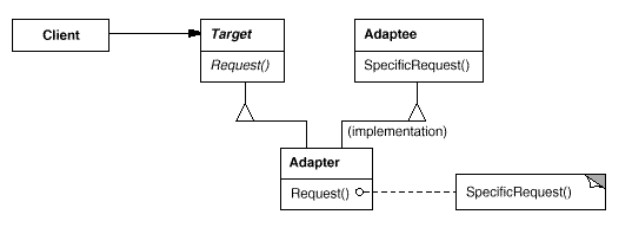
\includegraphics[scale=0.55]{imgs/class_adapter.jpg}
  \caption{Diagramma delle classi del pattern Class Adapter}
\end{figure}

Il Class Adapter adatta Adaptee a Target attraverso una specifica classe
concreta Adapter; questo non è sufficiente se si vuole adattare una classe
e tutte le sue sottoclassi. Per contro, però, permette di ridefinire parte del
comportamento di Adaptee con il subclassing, e introduce solamente un oggetto
(Adapter), senza ulteriore indirezione per raggiungere l'oggetto da adattare.

\paragraph{Object Adapter}
\label{par:object_adapter}

L'Object Adapter utilizza la composizione per adattare un'interfaccia ad
un'altra. Permette di adattare una classe e tutte le sue sottoclassi, ma rende
più difficoltoso modificare il comportamento dell'Adaptee.

\begin{figure}[h!]
  \centering
  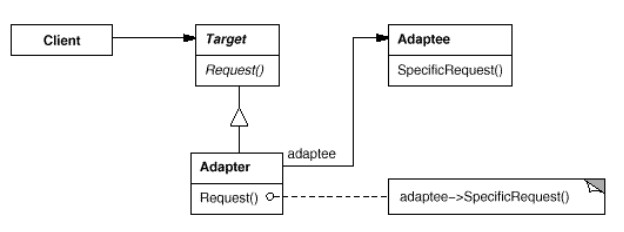
\includegraphics[scale=0.55]{imgs/object_adapter.jpg}
  \caption{Diagramma delle classi del pattern Object Adapter}
\end{figure}
